Several files (dynamic libraries, executables, drivers) were analyzed and reversed in order to achieve the aforementioned goals. However, the main analysis was performed in the {\bfseries ntoskrnl.exe} file, which is the one holding the actual implementation of the Windows Kernel.

It's important to stress that most of the general analysis was carried out using the Basic level of Telemetry. 

Further sections will depict different challenges and achievements faced during the analysis.




\section{Understanding how Telemetry makes use of ETW}
Where, who and what were some of the questions that needed to be answered in order to be able to get information about the providers that were registered against the DiagTrack session. 
It's possible to obtain the whole list of providers registered to a particular session, by executing the following powershell command: 

\begin{figure}[H]
  \begin{lstlisting}
    Get-EtwTraceProvider | where {$_.SessionName -match "<SESSION_NAME>"}
  \end{lstlisting} 
  \caption[]{Powershell comand to list ETW providers registered against a particular session. }
  \label{fig:powershell_cmd}
\end{figure}

One way to answer all the aforementioned questions, was to intercept the moment when some provider was going to write a message. If a breakpoint was set at that exact moment, it would be possible to gather information such as: 
\begin{enumerate}
\item The piece of code that triggered the write (by inspecting the call stack of the function).
\item The actual content of the log being written.
\end{enumerate} 
However, the function being used for executing writes ({\bfseries EtwWrite}) was not just used by the providers attached to the DiagTrack session but also by all the providers using the ETW framework. It was necessary to find a way to filter them and only intercept the ones important for the analysis. 

Using \ref{powershell_cmd}, it was possible to extract a GUID's list of the providers that were attached to the DiagTrack session. With this information, it would be possible to make the breakpoint to be triggered only when the provider's GUID that was trying to write was in the list. 

Nevertheless, this strategy had one minor issue. The function ({\bfseries EtwWrite}) had five parameters and none of them would show directly the GUID:

\begin{figure}[H]
  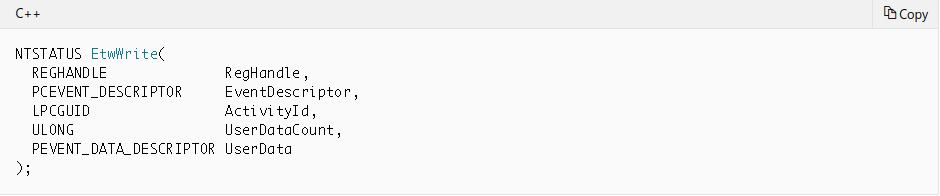
\includegraphics[width=\linewidth]{images/etw_write_docu.png}
  \caption[]{Documentation for EtwWrite function \footnote{https://docs.microsoft.com/en-us/windows-hardware/drivers/ddi/content/wdm/nf-wdm-etwwrite}. }
  \label{fig:etw_write_docu}
\end{figure}

The first parameter is the registration handler. This object is returned once the provider executed the registration ({\bfseries EtwRegister)} successfully.
On the other hand, the {\bfseries EtwRegister} receives the GUID as parameter:
\begin{figure}[H]
  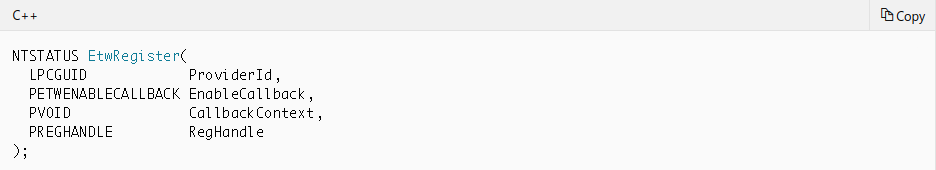
\includegraphics[width=\linewidth]{images/etw_register_docu.png}
  \caption[]{Documentation for EtwRegister function \footnote{https://docs.microsoft.com/en-us/windows-hardware/drivers/ddi/content/wdm/nf-wdm-etwregister}.}
  \label{fig:etw_register_docu}
\end{figure}

Therefore, in order to perform the cross-check it was not enough with information from the {\bfseries EtwWrite} function, but also information from the {\bfseries EtwRegister} was needed. To summarize, to understand if the write was being done by a provider registered against the DiagTrack session it was necessary to: 
\begin{enumerate}
    \item Extract the whole list of providers registered attached to the DiagTrack session.
    \item Intercept all the {\bfseries EtwRegister} executions and check if the GUID being used was inside the list.
    \item If it was, save the handler. 
    \item Intercept all the {\bfseries EtwWrite} executions and check if the handler being used is one of the stored handlers.
    \item If it was, the provider that is writing, is attached to the DiagTrack session.
\end{enumerate}

Even though the strategy seemed to be theoretically promising, it was necessary to understand how to actually carry out these actions. Further sections will depict that process.













\subsection{Reversing registration process}
As mentioned in section \ref{etw}, whenever a provider wants to register itself against a particular session, it has to call the function {\bfseries EtwWrite}.
Because of this, the first step was to analyze the behavior of this function, using {\bfseries IDA}(\ref{IDA}). As we can see in \ref{fig:etwRegsiter_code}, the only action being performed by {\bfseries EtwRegister}, was a call to another function named {\bfseries EtwpRegisterProvider}. 

\begin{centering}
\begin{figure}[H]
  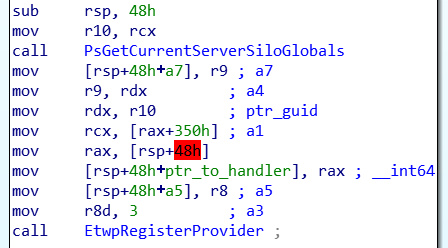
\includegraphics[width=12cm]{images/etwRegister_code.png}
  \caption[]{Dissasembly of ETWRegister function}
  \label{fig:etwRegister_code}
\end{figure}
\end{centering}

A quick analysis of the latter function showed that, apparently, this was the function holding the actual implementation of the registration process. However, due to the lack of documentation regarding this function, it was necessary to understand in a more in-depth way what was actually happening. Following chapters will present a detailed description of reversing (partially, only the interesting parts for this research) {\bfseries EtwpRegisterProvider}. 
To make it easier, it will be divided in different parts:
\begin{itemize}
  \item Understanding the layout of the function
  \item Check if a GUID for this provider already exists.
  \item If not found, create a new one.
  \item Create new entry and get the handler 
\end{itemize}





  \subsubsection{Understanding the layout of the function}
  {\bfseries EtwpRegisterProvider} received seven parameters:
  \begin{verbatim}
  signed __int64 __fastcall EtwpRegisterProvider(__int64 a1, _QWORD *a2,
        int a3, void (__fastcall *a4)(ULONG_PTR, __int64, __int128 *,
        __int64), __int64 a5, __int64 a6, __int64 *a7)
  \end{verbatim}

  Usually when performing reverse engineering, it is not necessary to understand every tiny detail, but only the key points that are important to meet the proposed goals. This wasn't the exception. 

  The main focus here was not to understand how the registration process fully worked but just to get an idea of it plus get to know the relation between GUID and registration handler.

  After understanding a little bit more about this function, it was possible to conclude that:
  \begin{enumerate}
  \item {\bfseries a1}: Is the pointer to a structure.
  \item {\bfseries a2}: Is the pointer to the GUID structure. 
  \item {\bfseries a7}: Is the address where the pointer to the registration handler will be placed (can be think as "function output").
  \end{enumerate}

  What is this {\bfseries a1} structure?
  The figure \ref{fig:etwRegister_code} shows that before calling {\bfseries EtwpRegisterProvider}, the function {\bfseries PsGetCurrentServerSiloGlobals} is invoked. This latter one returns a pointer to a structure $S$ of type {\bfseries \_ESERVERSILO\_GLOBALS}. 

  \begin{centering}
  \begin{figure}[H]
    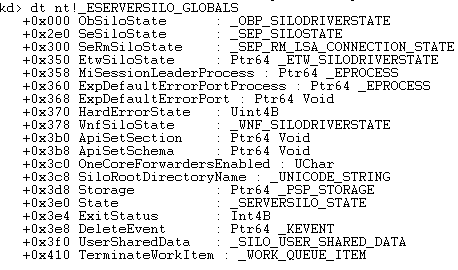
\includegraphics[width=12cm]{images/ESILOGLOBALS_structure.png}
    \caption[]{\_ESERVERSILO\_GLOBALS structure layout ($S$).}
    \label{fig:eserversilo_globals_structure}
  \end{figure}
  \end{centering}

  However, the first parameter provided to {\bfseries EtwpRegisterProvider} is not the pointer to $S$ but is the pointer to another structure $S_2$ of type {\bfseries \_ETW\_SILODRIVERSTATE}. which is part $S$, more precisely, it is situated at the offset 0x350. 

  \begin{centering}
  \begin{figure}[H]
    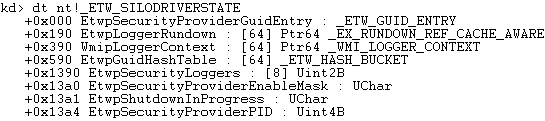
\includegraphics[width=12cm]{images/ETW_SILODRIVERSTATE_structure.png}
    \caption[]{\_ETW\_SILODRIVERSTATE structure layout ($S_2$).}
    \label{fig:etwsilodriverstate_structure}
  \end{figure}
  \end{centering}

  With all this information, was possible to conclude that {\bfseries a1} will point to a global structure holding configurations, settings and information in general directly related with the {\bfseries ETW} framework. In the other hand, {\bfseries a2} and {\bfseries a7} will hold pointers to a GUID and to a place were a registration handler will be placed afterwards, respectively. 
  With the knowledge of the purpose of just these three parameters, was possible to move forward.


  \subsubsection{Check if GUID for this provider already exists}
  Once inside the $EtwpRegisterProvider$ function, after performing some sanity checks, it tries to get the guid entry related with the GUID. If it doesn't exist, it will create one. 
  
  \begin{centering}
  \begin{figure}[H]
    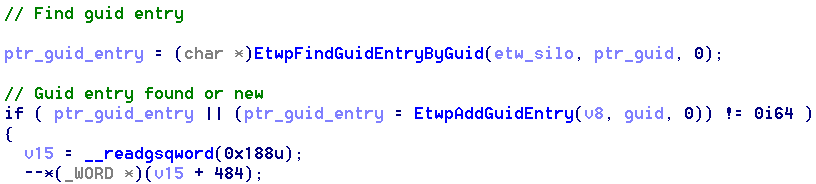
\includegraphics[width=15cm]{images/etwpregisterProvider.png}
    \caption[]{First lines of EtwpRegisterProvider}
    \label{fig:etwpregisterProvider}
  \end{figure}
  \end{centering}

  In this section, the focus will be on understanding how the process of recovering the already existing "GUID entry" works.

  The action of recovering is performed by a particular function called {\bfseries EtwpFindGuidEntryByGuid}:

  \begin{verbatim}
  ptr_guid_entry = (char *)EtwpFindGuidEntryByGuid(etw_silo, ptr_guid, 0);
  \end{verbatim}

  As can be inferred from the previous line, two important parameters are provided: the {\bfseries ETWSILODRIVERSTATE}(a1) structure $S$ and the pointer to the GUID $ptr\_guid$.

  \begin{centering}
  \begin{figure}[H]
    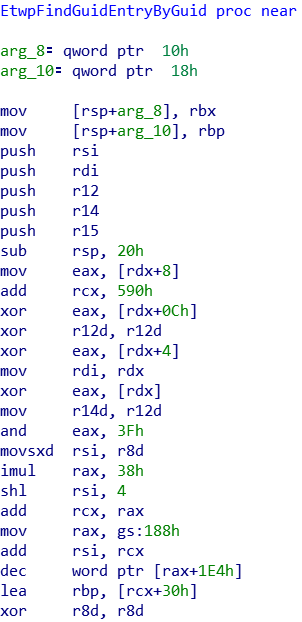
\includegraphics[width=6cm]{images/etwpfindentrybyguid1.png}
    \caption[]{First basic block of EtwpFindEntryByGuid.}
    \label{fig:EtwpFindEntryByGuid}
  \end{figure}
  \end{centering}

  Figure \ref{fig:etwsilodriverstate_structure} depicts how the function gets the guid entry related to the provider (if it exists). $rcx$ holds the pointer to $S$ and $rdx$ holds $ptr\_guid$.

  The first highlight is the $add$ function, which stores in $rcx$ the pointer to the structure stored at the offset $0x590$ of $S$. Going back to the structure layout of $S$ (figure \ref{fig:etwsilodriverstate_structure}), it can be appreciated that at the offset $0x590$, the structure $EtwpGuidHashTable$ of type $\_ETW\_HASH\_BUCKET[64]$ is present. Figure \ref{fig:etwhashbucketlayout} depicts its layout.

  Just before the $add$ function, $eax$ is filled with the content of the address $rdx+8$. $rdx$ held the $ptr\_guid$, meaning that $eax$ will have the third group of 4 bytes inside of the guid structure. Why the third? Because the offset was 8. Why 4 bytes? Because the register $eax$ (32 bits) was used.

  In the following lines, the value of $eax$ is being constantly modified by xoring it, successively with the different group of 4 bytes that compose the guid structure\footnote{Sometimes the structures weren't documented at all. Sometimes they were, but was not possible to find it until some kind of clue pointing to it was found.  So far the layout of the structure pointed by $ptr\_guid$ was unknown, however from this function it was possible to conclude that the structure had a size of 16 bytes.}. After performing this successive xor operations, an and function is applied against $eax$ using a mask of $0x3f$ and lastly multiplies the result of it against $0x38$ (size of $\_ETW\_HASH\_BUCKET$ structure). Finally, the value of $rax$($eax$) is added to $rcx$ which had the pointer to the $EtwpGuidHashTable$ structure. 

  Writing the aforementioned function in a pseudo-code style ($ptr$ is a short version of "pointer"): 
  \begin{verbatim}
  xor_guid_parts = ptr_guid[0] ^ ptr_guid[1] ^ ptr_guid[2] ^ ptr_guid[3]
  ptr_hash_table = ptr_S + 0x590
  ptr_bucket = ptr_hash_table + 0x38 * ((xor_guid_parts) & 0x3F) 
  \end{verbatim}

  Therefore, $ptr\_bucket$ is basically a pointer to a particular bucket inside the $EtwpGuidHashTable$, calculated based on the GUID of the provider. 
  Once this value is determined, a "look up" inside the structure is carried out in the following way:

  \begin{centering}
  \begin{figure}[H]
    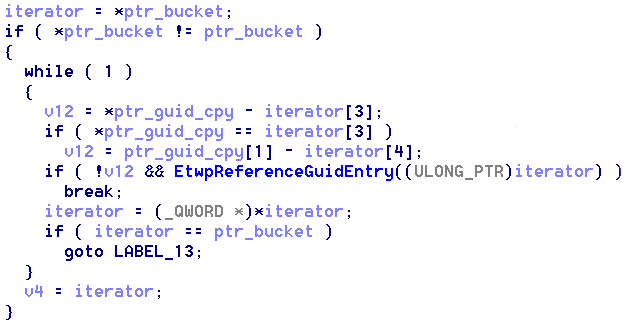
\includegraphics[width=12cm]{images/etwpfindentrybyguid_while.png}
    \caption[]{Part of EtwpFindEntryByGuid function extracted using IDA Hex-Rays plugin.}
    \label{fig:EtwpFindEntryByGuid_while}
  \end{figure}
  \end{centering}

  \begin{centering}
  \begin{figure}[H]
    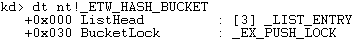
\includegraphics[width=10cm]{images/_etw_hash_bucket_structure.png}
    \caption[]{$\_ETW\_HASH\_BUCKET$ structure layout.}
    \label{fig:etwhashbucketlayout}
  \end{figure}
  \end{centering}

  At first an iterator is built. This iterator will point initially to the Flink of the first list entry\footnote{https://docs.microsoft.com/en-us/windows/desktop/api/ntdef/ns-ntdef-\_list\_entry} of the bucket (figure \ref{fig:etwhashbucketlayout}). The right-after if will capture the special case were the list is empty. In that particular case, the whole cycle will be skipped and the {\bfseries LABEL\_13} (routine to exit, which isn't displayed in the figure) will be executed. The only important thing of this routine is that it executes a return statement with the value of the variable $v4$ (which is initially defined as 0).

  If the list is not empty, the first operation which is carried out is a subtraction between the first quadword of the GUID and a value of $iterator[3]$. Due to the variable $iterator$ is defined as a 8-bytes pointer, $iterator[3]$ will point to the offset $0x18$ of the structure stored inside the Flink. In the case that both values are equal, the second comparison (between the second quadword of the GUID and the $iteartor[4]$) is carried out. 

  At this point some things can be concluded:
  \begin{itemize}
  \item The cycle is iterating a double-linked-list which holds a particular structure $T$.
  \item $T$ has the GUID of the provider stored at offset $0x18$
  \item Again, seems that the GUID is 16 bytes long.
  \item From the function name, it can concluded that $T$ is structure that represents the GUID entry.
  \end{itemize}

  Continuing with the code analysis, if some of the comparisons failed, the iterator changes its values to the next one in the list. Before continuing, it ensures that the cycle is not finished by checking if the actual value of the iterator is the same one used as the starting point. If they are equal, the exit routine is executed meaning that the return value will be 0.

  If both comparisons are equal (the GUID of the provider and the one stored in $T$ are the same), a function called $EtwpReferenceGuidEntry$ with the current value of the iterator as parameter, is called. After this execution, the cycle is finished by the break statement. However, before executing the exit routine, the value of $v4$ is filled up with the value of the $iterator$, meaning that the return value will be pointer to the guid entry related to the GUID of the provider. The $EtwpReferenceGuidEntry$ function just made some security checks not relevant for this task. \\

  Therefore, as a summary, it is possible to say that:\\
  {\bfseries The function $EtwpFindGuidEntryByGuid$ looks for a particular structure (most probably called guid entry), which is stored inside a double-linked-list of a bucket inside the $EtwpGuidHashTable$ of the $ETWSILODRIVERSTATE$, based on doing some mathematical operations with the GUID of the provider.}

  After finishing with this anlaysis, 
  












\subsubsection{If not found, create a new one}
In the previous section, it was explained how the 





\subsubsection{Create new entry and get the handler }

\newpage
{\huge 1. We couldn't ensure that the data was being written was actually going to the DiagTrack session .}

\section{When and how providers are registered}
\section{How writes are carried out}
\section{Relation between ETW session and ETW providers}
\section{Identifying the buffers}
\section{Provider GUID vs Group Provider GUID}
\section{Checking correctness of logged events}
\section{Automatization of event logging}
\section{Service isolation}
\section{Triggers}
\section{searching for new triggers} YARA
\section{Difference among configuration levels of telemtry}
\section{Analysis of sent data over the channel to Microsfot backend services}
